% !TeX spellcheck = en_US
\addsection{Map Elements}{\skills/logistics.png}

\bigskip

\begin{wrapfigure}{r}{0.5\textwidth}
  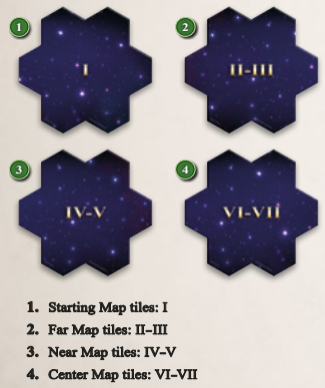
\includegraphics[width=0.9\linewidth]{\images/maptiles.png}
\end{wrapfigure}
Each Scenario is built using four types of Map Tiles.
Players always have a Faction-Specific Starting (I) Map Tile and may additionally have a number of face-down Far (II-III) Map Tiles which can be used to add new areas to the Scenario by spending MP.
Near (IV-V) and Center (VI-VII) Tiles are usually placed face down randomly during a Scenario’s setup and must be turned face up by spending MP when your Hero is next to them.
All face-down tiles should be selected randomly from the pool of possible Tiles and shuffled to keep their front side hidden.\par
The \textbf{roman numeral} of each tile describes the overall \textbf{difficulty of Neutral Units} on that tile, as well as the number of rewards players might expect to find on that Tile.
Starting (I) Tiles are the easiest while Center (VI-VII) Tiles are the most difficult.\par
\par

\begin{wrapfigure}{R}{0.5\textwidth}
  \begin{center}
  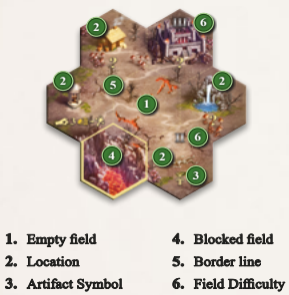
\includegraphics[width=0.47\textwidth]{\images/fields.png}
  \end{center}
\end{wrapfigure}
\subsection*{Map Tile Anatomy}
Each Map Tile is divided into 7 separate \textbf{Fields} that your Heroes can \textbf{Visit}.
When a Hero moves to a Field, they must immediately Visit it, or
first start a \hyperlink{Combat}{Combat} against the enemies guarding it before Visiting.
Empty Fields do nothing when Visited.
Solid yellow lines on a Field's edge cannot be passed through.
\hyperlink{Difficulty}{Roman numerals} written on a Field indicate that the Field is guarded by neutral enemies that must be fought to Visit it.\par

\clearpage

\begin{multicols}{2}

\subsection*{\hypertarget{Categories}{Location Categories}}
Visiting Fields provides Heroes with benefits such as gaining Resources or Cards.
There are three categories of Visitable Fields:
\begin{itemize}
  \item \textbf{Visitable} – Once you Visit this field, place a Black Cube on it.
    Treat it as an Empty Field as long as it has a Black Cube.
  \item \textbf{Flaggable} – These Fields can be directly captured by players and provide passive benefits.
    When you Visit one, place a Faction Cube on it and gain a benefit.
    Enemy Heroes who Visit your Flagged Fields will replace your Cube with theirs to \textbf{steal} the Field’s effects.
    Allied Heroes treat Flagged Fields \textbf{as if they were empty}.
  \item \textbf{Revisitable} – You can Visit this Field multiple times.
    Do not place a Black Cube when you Visit it.
    You may pay 1 MP to Visit this Field again when your Hero occupies this Field.
\end{itemize}

See \hyperlink{All}{this section} for a list of all possible Fields and what they do.
\subsection*{\hypertarget{Placing}{Placing and Discovering New Tiles}}
When you Hero is adjacent to an undiscovered face down Tile, that Hero may spend 1 MP during your turn to flip and reveal that Tile.
You may then rotate the Tile as you see fit and place it back face-up.\par
In some Scenarios you will receive your own individual stack of Far (II-III) Map Tiles.
These can be placed on the map to expand the play area.
Tiles should be kept \textbf{hidden from all players} until they are about to be placed.
Placing a new Tile costs 1MP.
It must be placed adjacent to the Hero who spends the MP, and to at least two other existing Tiles.
New Tiles must also be positioned so that there is a valid path that eventually joins them with all other Tiles.
You may always rotate Map Tiles when placing them.\par

\end{multicols}

\begin{figure*}[!hb]
  \centering
  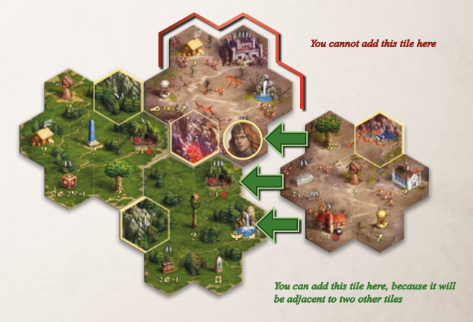
\includegraphics[width=\textwidth]{\images/placement.png}
\end{figure*}

\clearpage

\subsection*{Example}

\begin{multicols*}{2}

\textit{Sandro the Necromancer wants to capture an adjacent \hyperlink{Mines}{Mine} by Flagging it.
He spends a Movement Point to move onto the Mine, which begins \hyperlink{Combat}{Combat} against Neutral Units since the Field has a \hyperlink{Difficulty}{Difficulty Rating} and has not been previously Flagged by any player.}\par

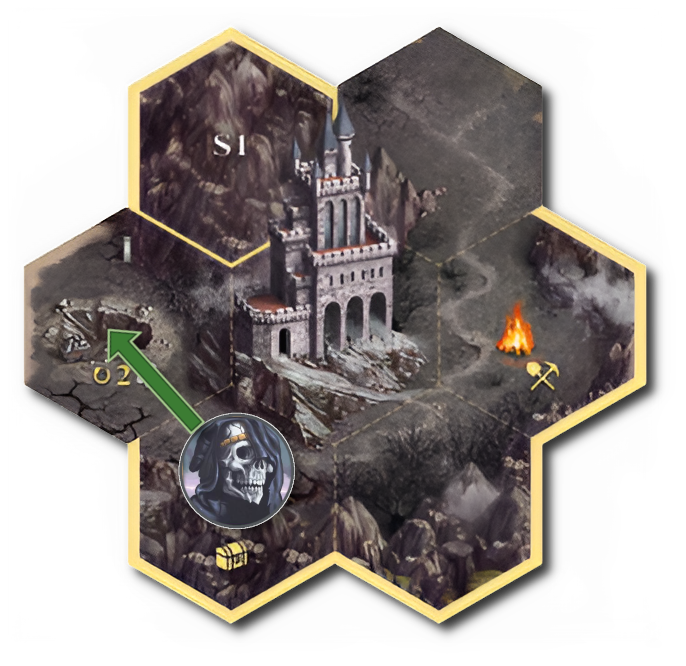
\includegraphics[width=1.1\linewidth]{\examples/sandro_takes_mine.png}

\textit{The Mine turns out to be guarded by Troglodytes, which have 3 HP \includesvg[height=0.8\baselineskip]{\svgs/health_points.svg}.
Sandro's current hand consists of a Power Card, a Lightning Bolt, Haste, and a Town Portal.
During the Combat, he casts the Lightning Bolt, and Empowers \includesvg[height=0.8\baselineskip]{\svgs/empower.svg} it with Haste's alternative (bottom) effect, which makes the Lightning Bolt deal 3 damage.}

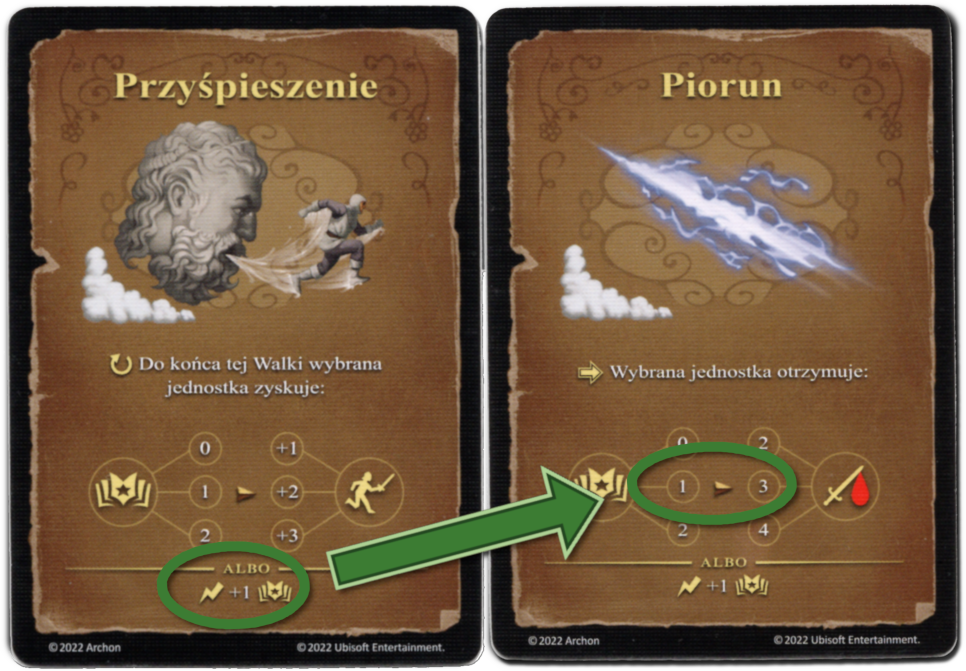
\includegraphics[width=\linewidth]{\examples/sandro_empowering_lightning_bolt.png}

\textit{
The Combat lasts for only one Round, so Sandro would not have been able to cast both Lightning Bolt and Haste, since players are limited to playing only one Spell Card per Combat Round.}\par


\textit{Sandro wins the Combat and Flags the Mine by placing one of his Faction Cubes on it.
Flagging this particular Mine increases his Building Materials \includesvg[height=0.8\baselineskip]{\svgs/building_materials.svg} production by 2, and he also immediately gains the Mine's production value of 2 \includesvg[height=0.8\baselineskip]{\svgs/building_materials.svg} as he was the first player to Flag it.}\par
\textit{Afterwards, Sandro wants to move back to a previously Flagged Settlement by casting the Town Portal still left in his hand.
He empowers it with the Power Card's Expert Effect \includesvg[height=0.8\baselineskip]{\svgs/expert.svg}, which grants him an additional Movement Point after casting it.
}

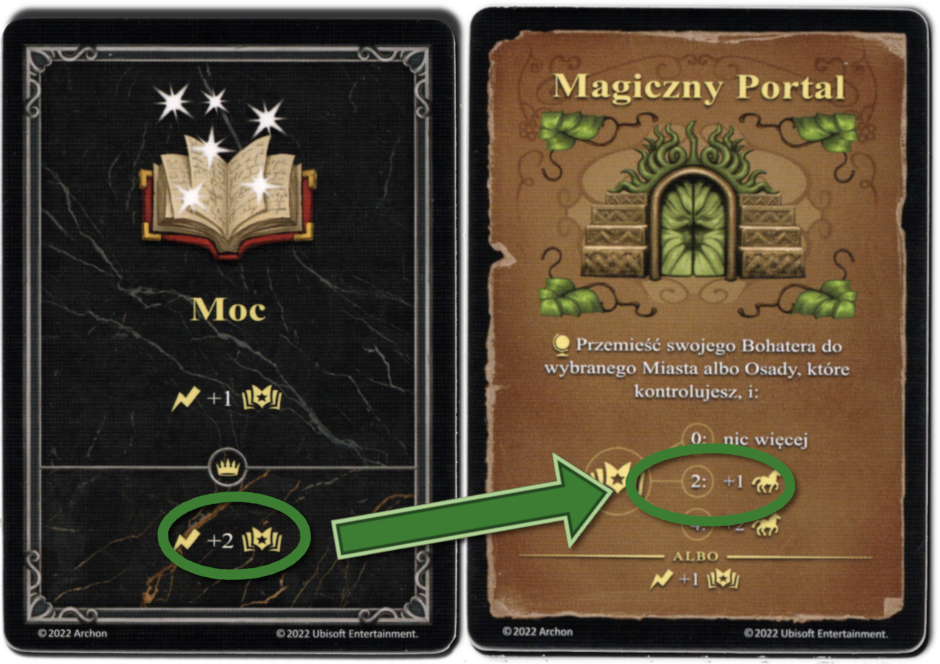
\includegraphics[width=\linewidth]{\examples/sandro_empowering_town_portal.png}

\textit{He is allowed to do this, as he is Level 2 and can thus use one \includesvg[height=0.8\baselineskip]{\svgs/expert.svg} each Game Round.}

\vfill
\hspace{2em}
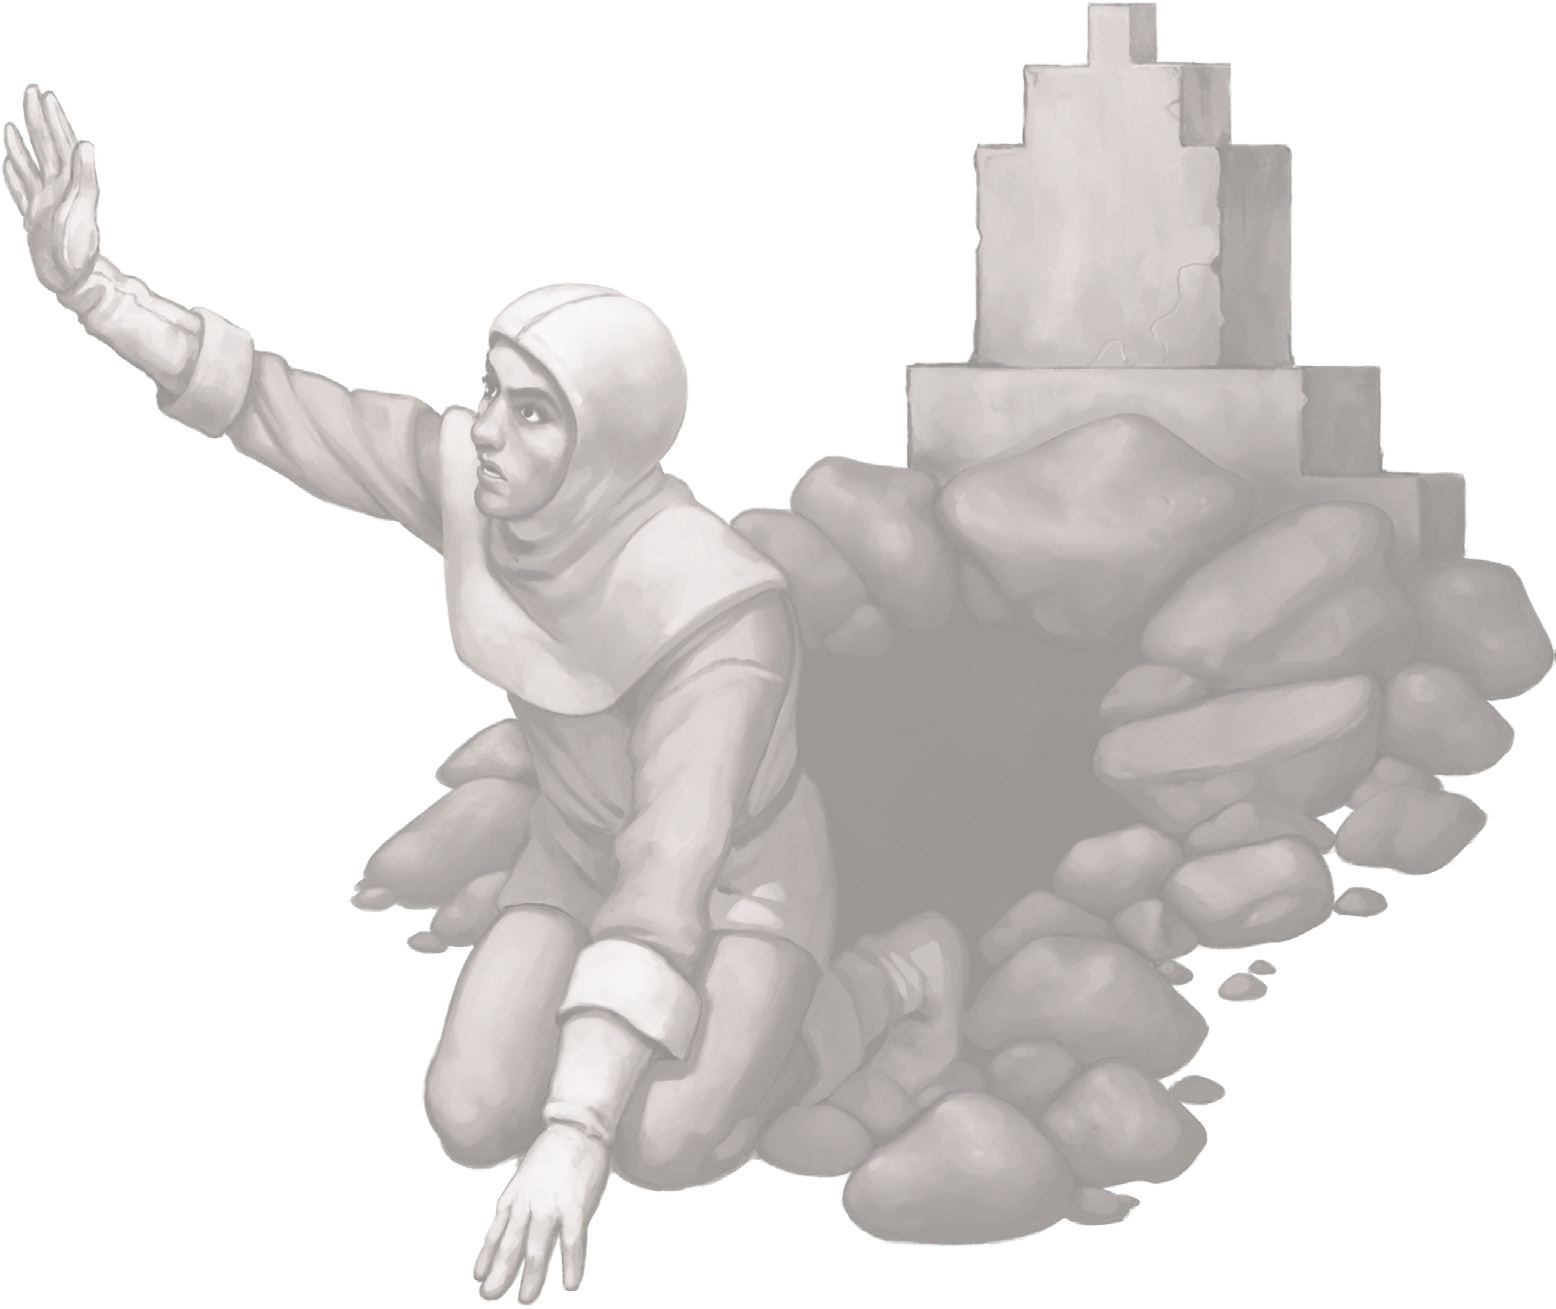
\includegraphics[width=\linewidth]{\art/resurrection.png}
\end{multicols*}
